\section{Detailed Negative Investigations}
\label{app:negative}

This appendix reports the two preregistered follow-ups summarized in Section~\ref{sec:negative}. Both work packages passed their validity, raw-reconstruction, dual-implementation, and artifact checks. Their scientific gates were negative.

\subsection{General additive token costs}
Let $\Xs=\prod_{i=1}^N\Xs_i$, let each $c_i$ be a metric with $\operatorname{diam}(c_i)\le1$, and define
\[
d_c(x,y)=\sum_{i=1}^N\lambda_i c_i(x_i,y_i),
\qquad \lambda_i>0,\quad \sum_i\lambda_i=1.
\]

\begin{theorem}[Product transport for additive coordinate costs]
\label{thm:general-additive}
If $P=\bigotimes_i p_i$ and $Q=\bigotimes_i q_i$ on finite supports, then
\[
W_{d_c}(P,Q)=\sum_i\lambda_iW_{c_i}(p_i,q_i).
\]
A product of coordinatewise $c_i$-optimal couplings attains the minimum.
\end{theorem}
\begin{proof}
For any coupling $\pi$ of $P$ and $Q$, its coordinate projection $\pi_i$ couples $p_i$ and $q_i$. Hence
\[
\Ex_\pi[d_c(X,Y)]
=\sum_i\lambda_i\Ex_{\pi_i}[c_i(X_i,Y_i)]
\ge\sum_i\lambda_iW_{c_i}(p_i,q_i).
\]
Conversely, finite support gives an optimal coordinate coupling $\pi_i^\star$ for every $i$. Their product couples $P$ and $Q$ and has expected cost equal to the lower bound.
\end{proof}

\begin{corollary}[General-cost first-divergence bound]
\label{cor:general-additive-fs}
For monotone mask-to-token copy-only chains and any valid path coupling $\Gamma$, at a deterministic horizon $r$,
\[
D_\Gamma^{(c)}(r)
\le \Ex_\Gamma\!\left[R_c(X_{\tau^{(r)}})\Ind{\tau^{(r)}\ne\dagger}\right],
\quad
R_c(s)=\sum_{i:s_i=\Mtok}\lambda_i\operatorname{diam}(c_i).
\]
\end{corollary}
\begin{proof}
Before the first split the chains share every committed token. Monotone copy-only evolution preserves those coordinates, so only coordinates still masked in the common pre-split state can differ at the endpoint; coordinate $i$ contributes at most $\lambda_i\operatorname{diam}(c_i)$.
\end{proof}

The empirical study fixes two alternatives without post-hoc tuning. The embedding hybrid is
$0.05\Ind{v\ne w}+0.95\|u_v-u_w\|_2/2$ for frozen normalized input-token embeddings; the byte hybrid replaces the Euclidean term with globally normalized byte-level Levenshtein distance.

\begin{table}[ht]
\caption{W8 CRN saturation. The alternatives change absolute scale but only slightly reduce the ratio to independent-FP variation.}
\label{tab:app-metric-saturation}
\centering\small
\begin{tabular}{@{}lrrr@{}}
\toprule
Metric & FP--W8 CRN & Independent FP & Saturation ratio \\
\midrule
Exact Hamming & 0.91455 & 0.97656 & 0.9365 \\
Embedding hybrid & 0.62349 & 0.67707 & 0.9209 \\
Tokenizer-byte hybrid & 0.06386 & 0.06972 & 0.9159 \\
\bottomrule
\end{tabular}
\end{table}

\begin{figure}[ht]
\centering
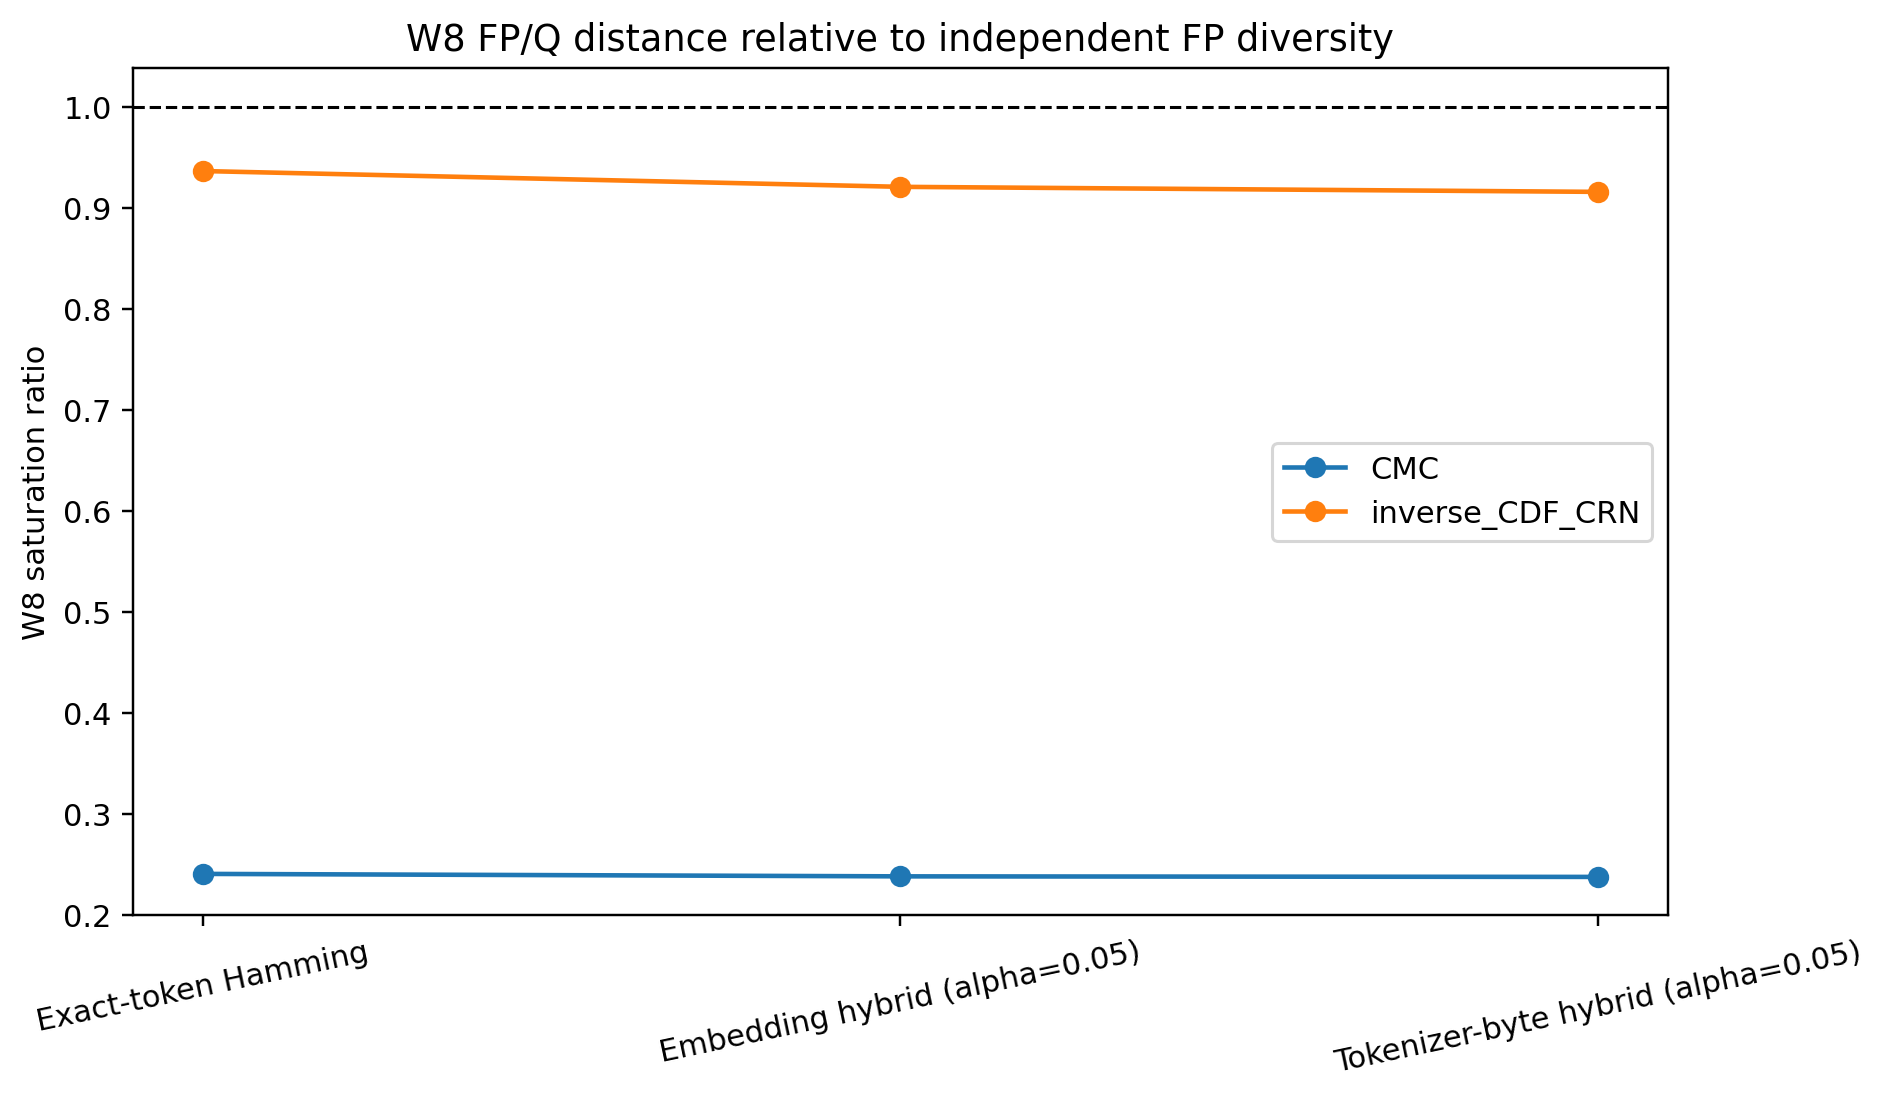
\includegraphics[width=.75\linewidth]{figures/figure_metric_saturation.png}
\caption{Alternative additive token costs do not materially de-saturate the W8 CRN comparison relative to independent-FP variation.}
\label{fig:app-metric-saturation}
\end{figure}

\begin{table}[ht]
\caption{Descriptive GSM8K relevance. The alternative metrics produce almost the same example ordering as Hamming.}
\label{tab:app-metric-task}
\centering\small
\begin{tabular}{@{}lrrr@{}}
\toprule
Metric & Answer-disagreement AUC & Correctness-disagreement AUC & Spearman vs. token edit \\
\midrule
Hamming & 0.9845 & \textbf{0.9573} & 0.99834 \\
Embedding hybrid & 0.9856 & 0.9532 & 0.99845 \\
Tokenizer-byte hybrid & \textbf{0.9876} & 0.9424 & 0.99846 \\
\bottomrule
\end{tabular}
\end{table}

\subsection{Held-out terminal lower-bound witnesses}
Coordinatewise Kantorovich potentials are trained on the fixed 64-prompt suite and frozen before evaluation on 128 disjoint prompt-population draws. The witness is 1-Lipschitz under the corresponding additive metric. A simultaneous empirical-Bernstein lower confidence bound uses the prompt block as the statistical unit.

\begin{table}[ht]
\caption{Held-out witness estimates and formal lower confidence bounds. All simultaneous LCBs are zero. Direct UCBs use the same retained evaluation prompt blocks.}
\label{tab:app-lower-bounds}
\centering\small
\begin{tabular}{@{}clrrr@{}}
\toprule
Bit & Metric & Witness estimate & Formal LCB & Direct CMC UCB \\
\midrule
W8 & Hamming & $-0.00049$ & 0 & 0.4256 \\
W8 & Embedding & $0.00083$ & 0 & 0.3380 \\
W8 & Byte & $-0.00008$ & 0 & 0.1617 \\
W6 & Hamming & $-0.00073$ & 0 & 0.5809 \\
W6 & Embedding & $0.00043$ & 0 & 0.4447 \\
W6 & Byte & $-0.00013$ & 0 & 0.1725 \\
W4 & Hamming & $0.05176$ & 0 & 0.9420 \\
W4 & Embedding & $0.02887$ & 0 & 0.6981 \\
W4 & Byte & $0.00361$ & 0 & 0.1969 \\
\bottomrule
\end{tabular}
\end{table}

\begin{figure}[ht]
\centering
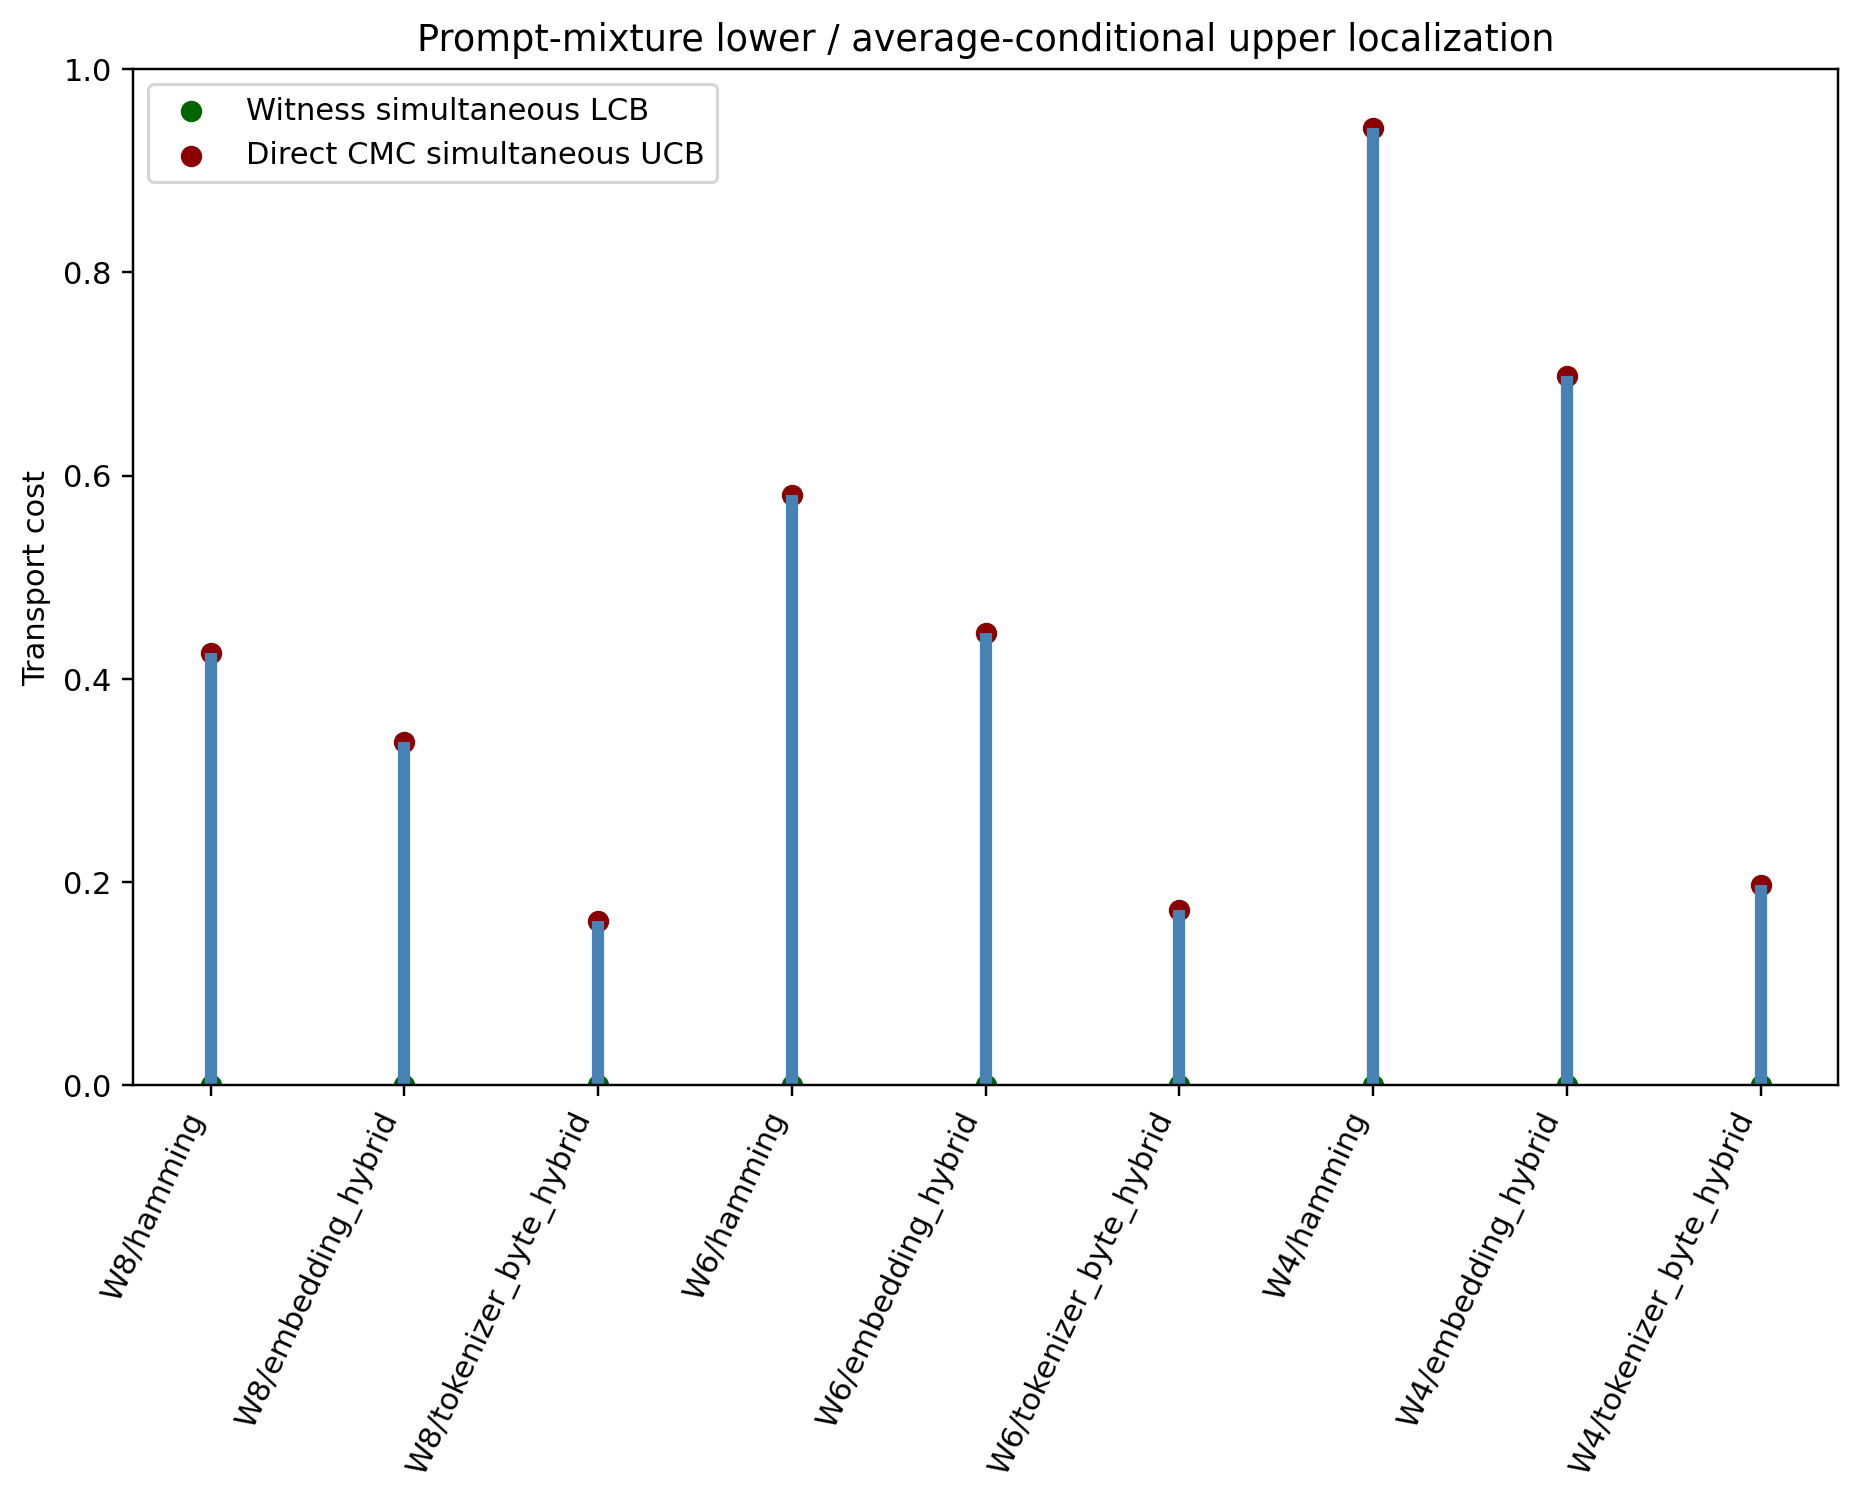
\includegraphics[width=.78\linewidth]{figures/figure_transport_localization.png}
\caption{The held-out point witnesses at W4 are positive, but distribution-free simultaneous lower confidence bounds remain zero. The experiment therefore does not localize terminal Wasserstein distance away from zero.}
\label{fig:app-localization}
\end{figure}

\subsection{Transport-weighted clipping calibration}
The calibration pilot evaluates per-output-row clipping selected with uniform, margin-frontier, residual-only, hazard-only, survival--residual (SR), and survival--residual--hazard (SRH) state weights. The primary W4 endpoint is exact GSM8K accuracy on 512 held-out examples. All methods use the same clipping grid, module set, prompt split, and quantization contract.

\begin{figure}[ht]
\centering
\begin{minipage}[t]{.55\linewidth}
\centering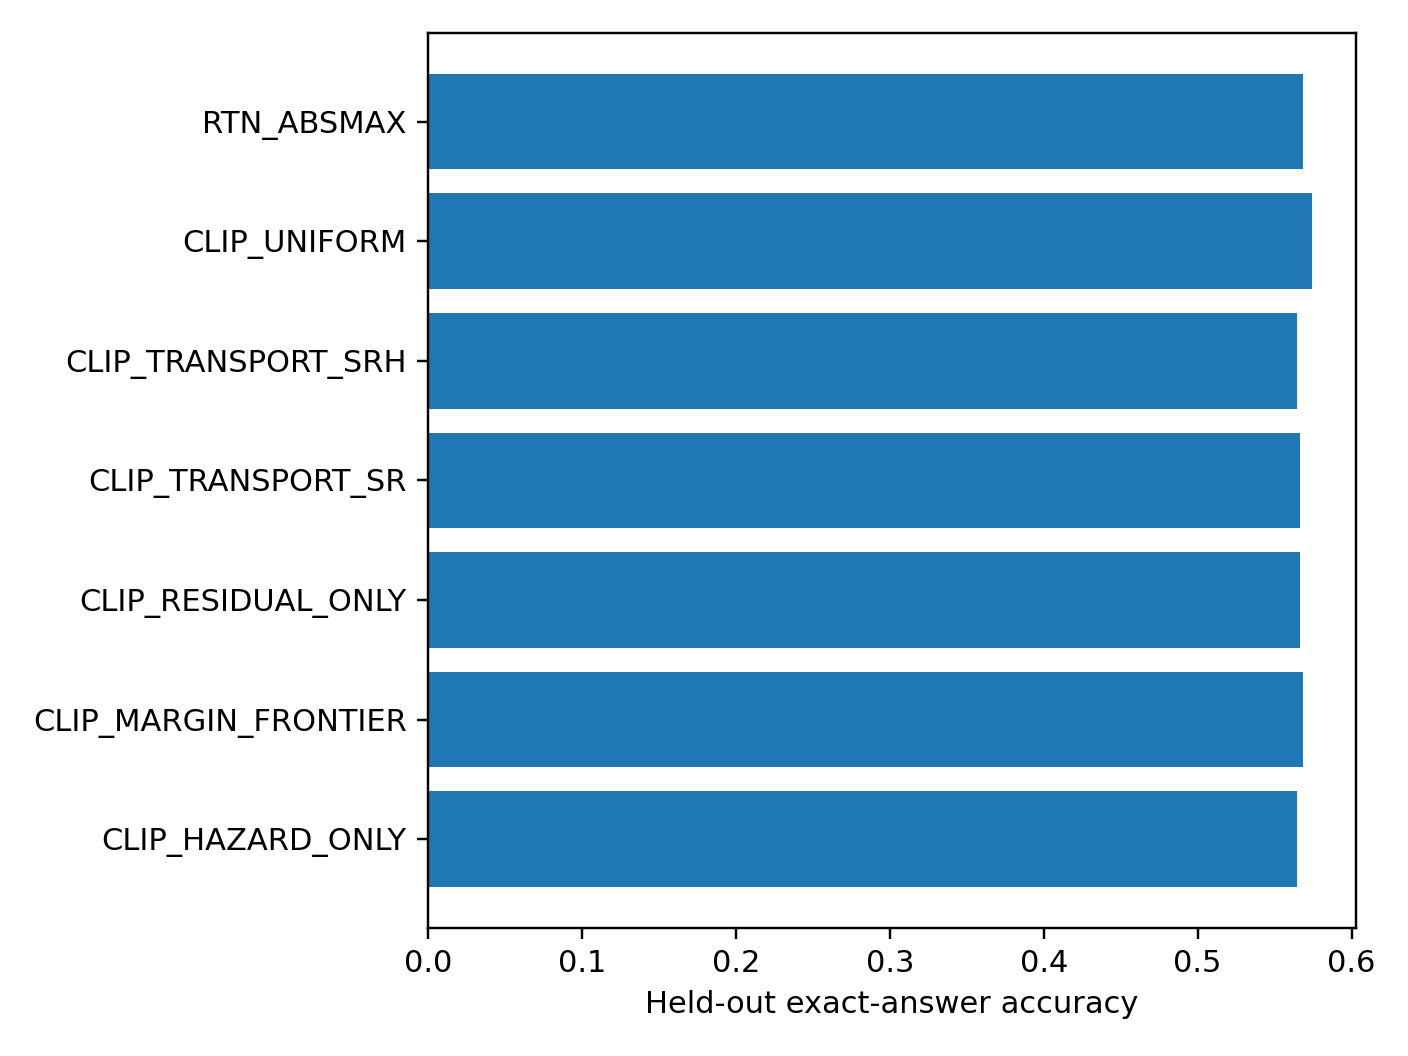
\includegraphics[width=\linewidth]{figures/figure_trcal_w4_accuracy.png}
\end{minipage}\hfill
\begin{minipage}[t]{.42\linewidth}
\centering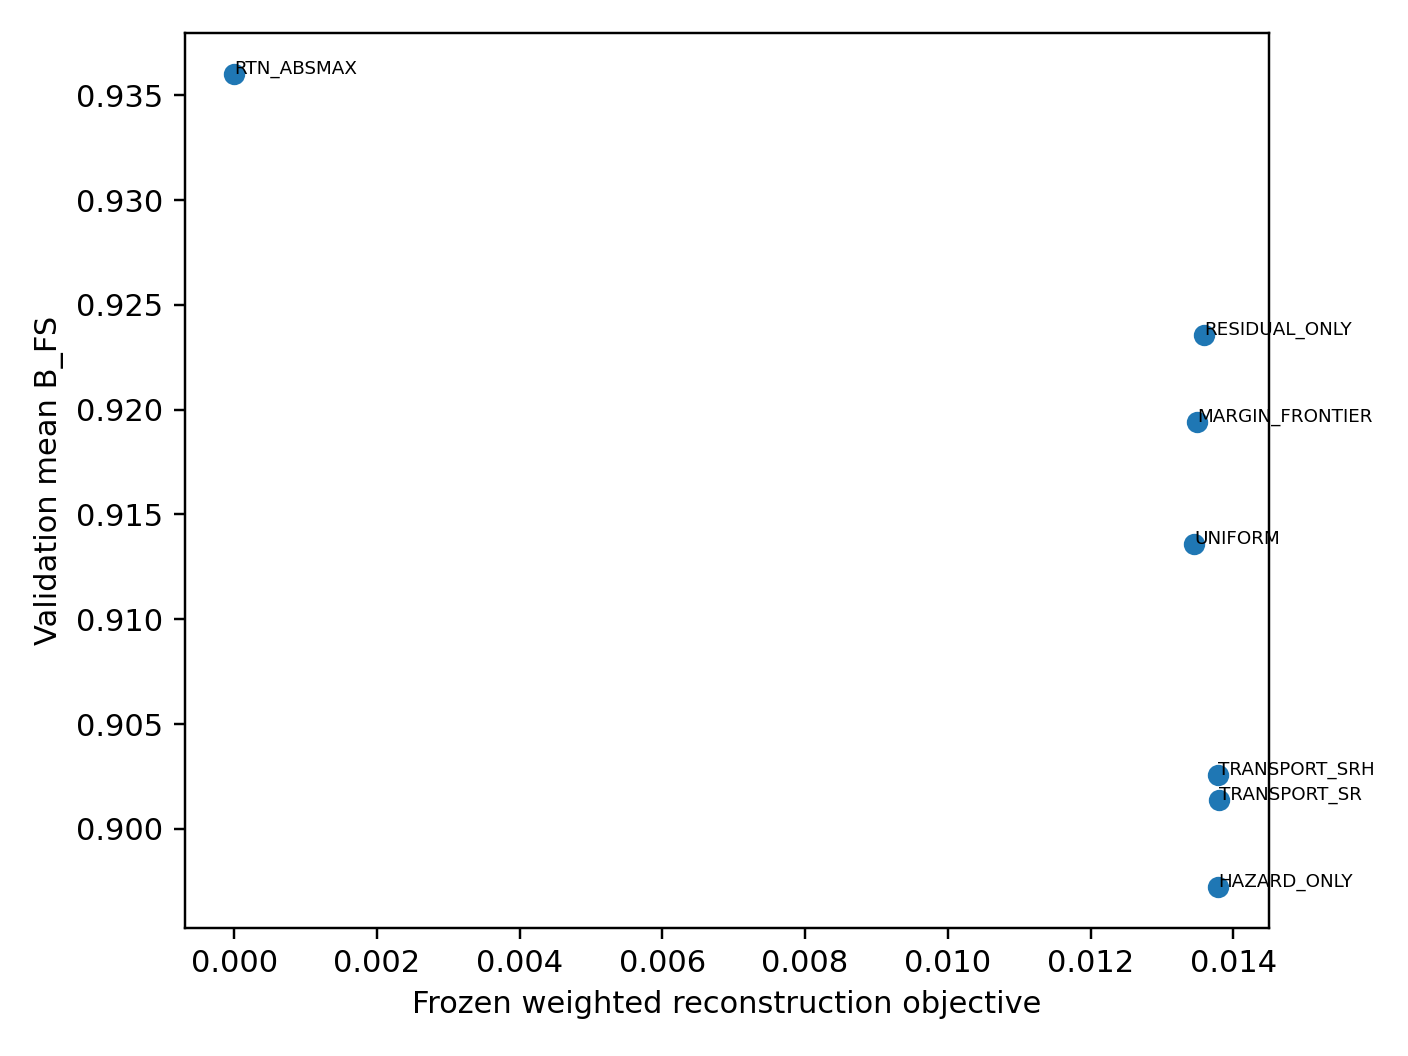
\includegraphics[width=\linewidth]{figures/figure_trcal_bridge.png}
\end{minipage}
\caption{\textbf{Left:} transport-weighted clipping does not improve the primary W4 task endpoint over uniform clipping. \textbf{Right:} the local reconstruction surrogate weakly predicts the next split.}
\label{fig:app-trcal}
\end{figure}

\begin{table}[ht]
\caption{Primary paired W4 comparisons for Transport SR.}
\label{tab:app-trcal-paired}
\centering\small
\begin{tabular}{@{}lrrr@{}}
\toprule
Comparator & Accuracy difference & 95\% paired-bootstrap interval & One-sided McNemar $p$ \\
\midrule
RTN absmax & $-0.20$ pp & $[-1.95,1.37]$ pp & 0.676 \\
Uniform clipping & $-0.78$ pp & $[-1.95,0.39]$ pp & 0.945 \\
Margin frontier & $-0.20$ pp & $[-1.17,0.78]$ pp & 0.773 \\
\bottomrule
\end{tabular}
\end{table}

Transport SR reduces terminal Hamming from $0.0534$ under RTN to $0.0381$ and increases BF16 answer agreement from $84.57\%$ to $89.26\%$, but ground-truth accuracy does not improve. Relative to uniform clipping, it has lower Hamming but lower accuracy and slightly higher $B_{\rm FS}$. The state-level surrogate audit gives split-prediction ROC AUC $0.545$ with interval $[0.479,0.602]$ and Spearman correlation $0.052$ with residual terminal damage. At W3, clipping methods substantially improve over absmax RTN, but SR/SRH are not uniquely better than uniform or margin-frontier calibration.

\subsection{Interpretation}
The negative findings rule out specific stronger stories, not the primary framework. The tested static token costs are not semantic metrics; the frozen prompt-independent witness does not yield a positive population LCB; and the tested local reconstruction objective does not reliably proxy first-split risk. Accordingly, no claim is made that the framework identifies the true terminal Wasserstein distance, supplies a task-improving quantizer, or certifies semantic quality.
